\documentclass[sigconf,authorversion]{acmart}

\usepackage{xcolor}

\usepackage[ruled]{algorithm2e}
\usepackage{multirow}
\renewcommand{\algorithmcfname}{ALGORITHM}

\usepackage{amssymb,amsbsy}
\usepackage{bbm}
\usepackage{paralist}
\usepackage{placeins}
\usepackage{tikz}
\usepackage{pgfplots}
\usepackage{pgfplotstable}
\usepackage{balance}
\usepackage{hyphenat} 
\pgfplotsset{compat=newest,scaled y ticks=false}
\usepgfplotslibrary{groupplots}
\usetikzlibrary{shapes}
\pgfplotsset{scaled y ticks=false,
  yticklabel style={
        /pgf/number format/fixed,
        /pgf/number format/precision=4
  },
}

\def\BibTeX{{\rm B\kern-.05em{\sc i\kern-.025em b}\kern-.08emT\kern-.1667em\lower.7ex\hbox{E}\kern-.125emX}}



\newcommand{\KL}[2]{\mathrm{KL}\left(#1 \middle\| #2\right)}

\def\amax{\mathrm{arg\,max}}
\def\amin{\mathrm{arg\,min}}
\def\knn{\mathrm{kNN}}
\def\fro{\mathrm{Fro}}
\def\RMSE{\mathrm{RMSE}}
\def\recvae{\mathrm{RecVAE}}
\def\SS{{\bf S}}
\def\bs{{\bf s}}
\def\x{{\bf x}}
\def\XX{{\bf X}}
\def\KK{{\bf K}}
\def\UU{{\bf U}}
\def\CC{{\bf C}}
\def\VV{{\bf V}}
\def\DD{{\bf D}}
\def\BB{{\bf B}}
\def\bZero{{\bf 0}}
\def\AA{{\bf A}}
\def\RR{{\bf R}}
\def\y{{\bf y}}
\def\bt{{\bf t}}
\def\d{\mathrm{d}}
\def\ba{{\bf a}}
\def\bw{{\bf w}}
\def\bu{{\bf u}}
\def\bp{{\bf p}}
\def\bt{{\bf t}}
\def\bm{{\bf m}}
\def\bz{{\bf z}}
\def\bv{{\bf v}}
\def\bc{{\bf c}}
\def\br{{\bf r}}
\def\bh{{\bf h}}
\def\bi{{\bf i}}
\def\bbf{{\bf f}}
\def\by{{\bf y}}
\def\bo{{\bf o}}
\def\E{{\bf E}}
\def\bI{{\bf I}}
\def\M{{\cal M}}
\def\N{{\mathcal N}}
\def\B{{\cal B}}
\def\Mult{\mathrm{Mult}}
\def\bb{{\bf b}}
\def\RR{{\mathbb R}}
\def\I{{\bf I}}
\def\dec{\mathrm{dec}}
\def\enc{\mathrm{enc}}
\def\boldeta{{\boldsymbol{\eta}}}
\def\btheta{{\boldsymbol{\theta}}}
\def\bmu{{\boldsymbol{\mu}}}
\def\bsigma{{\boldsymbol{\sigma}}}
\def\bphi{{\boldsymbol{\phi}}}
\def\bpi{{\boldsymbol{\pi}}}
\def\beps{{\boldsymbol{\epsilon}}}
\def\wsup{\ensuremath{W_{\mathrm{sup}}}}
\def\bz{\boldsymbol{z}}
\def\bOne{\boldsymbol{1}}
\def\bw{\boldsymbol{w}}
\def\bx{\boldsymbol{x}}
\def\dtest{{D_{\mathrm{test}}}}
\def\ppx{\mathrm{perplexity}}
\def\glm{\mathrm{GLM}}
\def\tw{{\tilde w}}
\def\tb{{\tilde b}}
\def\tbx{{\tilde \bx}}
\def\tbw{{\tilde \bw}}
\def\tby{{\tilde \by}}
\def\bbv{{\bar \bv}}
\def\maf{\mathrm{MAF}}
\def\bcl{{\bar\bc}}

\copyrightyear{2020}
\acmYear{2020}
\setcopyright{acmlicensed}
\acmConference[WSDM '20]{The Thirteenth ACM International Conference on Web Search and Data Mining}{February 3--7, 2020}{Houston, TX, USA}
\acmBooktitle{The Thirteenth ACM International Conference on Web Search and Data Mining (WSDM '20), February 3--7, 2020, Houston, TX, USA}
\acmPrice{15.00}
\acmDOI{10.1145/3336191.3371831}
\acmISBN{978-1-4503-6822-3/20/02}

\settopmatter{printacmref=true}
\begin{document}

\title{RecVAE: a New Variational Autoencoder for Top-N Recommendations with Implicit Feedback}

\author{Ilya Shenbin}
\email{ilya.shenbin@gmail.com}
\affiliation{
  \institution{Samsung-PDMI Joint AI Center, Steklov Institute of Mathematics at St.~Petersburg, Russia}
}

\author{Anton Alekseev}
\email{anton.m.alexeyev@gmail.com}
\affiliation{
  \institution{Samsung-PDMI Joint AI Center, Steklov Institute of Mathematics at St.~Petersburg, Russia}
}

\author{Elena Tutubalina}
\email{tutubalinaev@gmail.com}
\affiliation{
  \institution{Samsung-PDMI Joint AI Center, Steklov Institute of Mathematics at St.~Petersburg, Russia}
}

\author{Valentin Malykh}
\email{valentin.malykh@phystech.edu}
\affiliation{
  \institution{Neural Systems and Deep Learning Laboratory, Moscow Institute of Physics and Technology, Russia}
}

\author{Sergey I. Nikolenko}
\email{sergey@logic.pdmi.ras.ru}
\affiliation{
  \institution{Samsung-PDMI Joint AI Center, Steklov Institute of Mathematics at St.~Petersburg, Russia}
}

\renewcommand{\shortauthors}{Shenbin et al.}

\begin{abstract}
Recent research has shown the advantages of using autoencoders based on deep neural networks for collaborative filtering. In particular, the recently proposed \emph{Mult-VAE} model, which used the multinomial likelihood variational autoencoders, has shown excellent results for top-N recommendations. In this work, we propose the \emph{Recommender VAE} (RecVAE) model that originates from our research on regularization techniques for variational autoencoders. \emph{RecVAE} introduces several novel ideas to improve \emph{Mult-VAE}, including a novel composite prior distribution for the latent codes, a new approach to setting the  hyperparameter for the -VAE framework, and a new approach to training based on alternating updates. In experimental evaluation, we show that \emph{RecVAE} significantly outperforms previously proposed autoencoder-based models, including \emph{Mult-VAE} and \emph{RaCT}, across classical collaborative filtering datasets, and present a detailed ablation study to assess our new developments. Code and models are available at \urlstyle{tt}\url{https://github.com/ilya-shenbin/RecVAE}.
\end{abstract}

\begin{CCSXML}
<ccs2012>
<concept>
<concept_id>10010147.10010257.10010293.10010300.10010305</concept_id>
<concept_desc>Computing methodologies~Latent variable models</concept_desc>
<concept_significance>500</concept_significance>
</concept>
<concept>
<concept_id>10010147.10010257.10010282.10010292</concept_id>
<concept_desc>Computing methodologies~Learning from implicit feedback</concept_desc>
<concept_significance>300</concept_significance>
<concept>
<concept_id>10010147.10010257.10010321.10010337</concept_id>
<concept_desc>Computing methodologies~Regularization</concept_desc>
<concept_significance>300</concept_significance>
</concept>
<concept>
<concept_id>10010147.10010257.10010293.10010294</concept_id>
<concept_desc>Computing methodologies~Neural networks</concept_desc>
<concept_significance>100</concept_significance>
</concept>
<concept>
<concept_id>10002951.10003317.10003338.10003343</concept_id>
<concept_desc>Information systems~Learning to rank</concept_desc>
<concept_significance>300</concept_significance>
</concept>
</ccs2012>
\end{CCSXML}

\ccsdesc[500]{Computing methodologies~Latent variable models}
\ccsdesc[300]{Computing methodologies~Learning from implicit feedback}
\ccsdesc[300]{Computing methodologies~Regularization}
\ccsdesc[100]{Computing methodologies~Neural networks}
\ccsdesc[300]{Information systems~Learning to rank}

\keywords{deep learning, collaborative filtering, variational autoencoders}

\maketitle

\section{Introduction}

Matrix factorization (\emph{MF}) has become the industry standard as the foundation of recommender systems based on collaborative filtering. However, there are certain general issues that arise with this family of models. First, the number of parameters in any matrix factorization model is huge: it linearly depends on the number of both users and items, which leads to slow model learning and overfitting. Second, to make a prediction for a new user/item based on their ratings, one has to run an optimization procedure in order to find the corresponding user/item embedding. Third, only a small amount of ratings are known for some (often for a majority of) users and items, which could also lead to overfitting. This makes it necessary to heavily regularize matrix factorization models, and standard  or  regularizers are hard to tune.

Recently proposed models such as the \emph{Collaborative Denoising Autoencoder} (\emph{CDAE})~\cite{wu2016collaborative} partially solve these issues by using a parameterized function which maps user feedback to user embeddings. It performs regularization in an alternative way and makes it possible to predict item ratings for new users without additional iterative training. The \emph{Variational Autoencoder for Collaborative Filtering} (Mult-VAE)~\cite{liang2018variational} is a subsequent improvement of \emph{CDAE} that extends it to multinomial distributions in the likelihood, which are more suitable for recommendations.

In this work, we propose the \emph{Recommender VAE} (RecVAE) model for collaborative filtering with implicit feedback based on the variational autoencoder (VAE) and specifically on the \emph{Mult-VAE} approach. \emph{RecVAE} presents a number of important novelties that together combine into significantly improved performance. First, we have designed a new architecture for the encoder network. Second, we have introduced a novel composite prior distribution for the latent code  in the variational autoencoder. The composite prior is a mixture of a standard Gaussian prior and the latent code distribution with parameters fixed from the previous iteration of the model (Section~\ref{sec:prior}), an idea originating from reinforcement learning where it is used to stabilize training~\cite{DBLP:journals/corr/SchulmanWDRK17,houthooft2016vime}. In the context of recommendations, we have also found that this prior improves training stability and performance. Third, we have developed a new approach to setting the hyperparameter  for the Kullback-Leibler term in the objective function (Section~\ref{sec:kl}). We have found that  should be user-specific, , and should depend on the amount of data (implicit feedback) available for a given user.

Finally, we introduce a novel approach for training the model. In \emph{RecVAE}, training is done by alternating updates for the encoder and decoder (see Section~\ref{sec:als}). This approach has two important advantages. First, it allows to perform multiple updates of the encoder (a more complex network) for every update of the decoder (a very simple, single-layer network that contains item embeddings and biases). Second, it allows to use corrupted inputs (following the general idea of denoising autoencoders~\cite{im2017denoising,shu2018amortized}) only for training the encoder while still training the decoder on clean input data. This is again beneficial for the final model training due to the differing complexities of the encoder and decoder. 

As a result of the above novelties, our model significantly outperforms all autoencoder-based previous works and shows competitive or better results in comparison with other models across a variety of collaborative filtering datasets, including \emph{MovieLens-20M} (ML-20M), \emph{Netflix Prize Dataset}, and \emph{Million Songs Dataset} (MSD).

The paper is organized as follows. In Section~\ref{sec:background} we review the crucial components and approaches we are to employ in the proposed methods as well as other relevant prior art.
In Section~\ref{sec:method} we describe the basic \emph{Mult-VAE} approach and our modifications. Section~\ref{sec:experiments} contains the results of a comprehensive experimental study for our model, 
and Section~\ref{sec:conclusion} concludes the paper.

\section{Background and related work}\label{sec:background}

\subsection{Variational autoencoders and their extensions}\label{sec:vae}

The \emph{variational autoencoder} (VAE)~\cite{DBLP:journals/corr/KingmaW13,DBLP:conf/icml/RezendeMW14} is a deep latent variable model able to learn complex distributions. We begin with a brief exposition of the basic assumptions behind VAE that have been extended for collaborative filtering in \emph{Mult-VAE} and will be further extended in this work with \emph{RecVAE}. First, under the assumption that the dataset belongs to a low-dimensional manifold embedded in a high-dimensional space, the marginal likelihood function can be expressed via a latent code  as . Since the marginal likelihood function is intractable, it is usually approximated with the evidence lower bound (ELBO):


\noindent
where  is the Kullback-Leibler divergence,  is the prior distribution,  is a variational approximation of the posterior distribution defined as a parameterized function with , and  are the parameters of . This technique, known as \emph{amortized inference}, provides additional regularization and allows to obtain variational parameters with a closed form function. 

Variational autoencoders can be used not only as generative models but also for representation learning. -VAE~\cite{higgins2017beta} is a modification of VAE designed to learn so-called \emph{disentangled representations} by adding a regularization coefficient to the Kullback-Leibler term in the evidence lower bound. The objective function of -VAE can still be considered as a valid ELBO with additional approximate posterior regularization that rescales the Kullback-Leibler divergence in formula~\eqref{eq:elbo_vae} above by a factor of~~\cite{hoffman2017beta,DBLP:conf/icml/MathieuRST19}:


\emph{Denoising variational autoencoders} (DVAE)~\cite{im2017denoising,shu2018amortized}, similar to denoising autoencoders, are trying to reconstruct the input from its corrupted version. The ELBO in this model is defined as


\noindent
It differs from VAE by the additional expectation , where  is a noise distribution, usually Bernoulli or Gaussian. Similar to how denoising autoencoders are more robust and generalize better than regular autoencoders, DVAE improves over the performance of the basic VAE and makes it possible to learn more robust approximate posterior distributions.

The \emph{Conditional Variational Autoencoder} (CVAE)~\cite{sohn2015learning} is another VAE extension which is able to learn complex conditional distributions. Its ELBO is as follows:


which is the same as the ELBO for regular VAE shown in~\eqref{eq:elbo_vae} but with all distributions conditioned on . \emph{VAE with Arbitrary Conditioning} (VAEAC) \cite{DBLP:conf/iclr/IvanovFV19}, based on CVAE, solves the imputation problem for missing features, which is in many ways similar to collaborative filtering. It has an ELBO similar to~\eqref{eq:elbo_cvae} where the variable are the unobserved features  and the condition is  for some binary mask :

an important point here is that the mask  can be different and even have different number of ones (unobserved features) for different inputs . However, this approach cannot be directly applied to the implicit feedback case, which we consider in this work.

\subsection{Autoencoders and Regularization for Collaborative Filtering}\label{sec:ae_cf}

Let  and  be the sets of users and items respectively in a collaborative filtering problem. Consider the implicit feedback matrix , where  if the th user positively interacted with (liked, bought, watched etc.) the th item (movie, good, article etc.) and  otherwise. We denote by  the feedback vector of user .

The basic idea of the \emph{Collaborative Denoising Autoencoder} (\emph{CDAE}) model~\cite{wu2016collaborative} is to reconstruct the user feedback vector  from its corrupted version . The corrupted vector  is obtained by randomly removing (setting to zero) some values in the vector~. The encoder part of the model maps  to the hidden state. In CDAE, both encoder and decoder are single neural layers (so the model itself is basically a feedforward neural network with one hidden layer), with a user input node providing user-specific weights and the rest of the weights shared across all users; the latent representation  and reconstructed feedback  are computed as

where  and  are input-to-hidden and hidden-to-output weight matrices respectively, and  is the weight vector for the user input node). Note that the matrix  can be considered as a matrix of item embeddings, and the matrix , as the matrix of user embeddings.

Previous work also indicates that regularization plays a central role in collaborative filtering. Models based on matrix factorization (MF) with user/item embeddings almost invariably have an extremely large number of parameters that grows with dataset size; even a huge dataset with user ratings and other kinds of feedback cannot have more than a few dozen ratings per user (real users will not rate more items than that), so classical MF-based collaborative filtering models require heavy regularization~\cite{Park:2012:LRC:2181339.2181690,bell2007scalable,Adomavicius:2005:TNG:1070611.1070751}. The standard solution is to use simple  or  regularizers for the embedding weights, although more flexible priors have also been used in literature~\cite{salakhutdinov2008bayesian,lawrence2009non}. The works~\cite{wu2016collaborative,liang2018variational} present an alternative way of regularization based on the amortization of user embeddings coupled with denoising~\cite{vincent2010stacked,im2017denoising,shu2018amortized}. Several more models are reviewed in Section \ref{sec:baselines}.

The model which is nearest to our current work in prior art is \emph{Multinomial VAE} (\emph{Mult-VAE})~\cite{liang2018variational}, an extension of variational autoencoders for collaborative filtering with implicit feedback. In the next section, we begin with a detailed description of this model and then proceed to presenting our novel contributions.


\section{Proposed approach}\label{sec:method}

\subsection{Mult-VAE}\label{sec:mult}

We begin with a description of the \emph{Mult-VAE} model proposed in~\cite{liang2018variational}. The basic idea of \emph{Mult-VAE} is similar to VAE but with the multinomial distribution as the likelihood function instead of Gaussian and Bernoulli distributions commonly used in VAE. The generative model samples a -dimensional latent representation  for a user , transforms it with a function  parameterized by~, and then the feedback history  of user , which consists of  interactions (clicks, purchases etc.), is assumed to be drawn from the multinomial distribution:

Note that classical collaborative filtering models also follow this scheme with a linear ; the additional flexibility of \emph{Mult-VAE} comes from parameterizing  with a neural network with parameters .

To estimate  one has to approximate the intractable posterior . This, similar to regular VAE, is done by constructing an evidence lower bound for the variational approximation where  is assumed to be a fully factorized diagonal Gaussian distribution: . The resulting ELBO is


which follows the general VAE structure with an additional hyperparameter  that allows to achieve a better balance between latent code independence and reconstruction accuracy, following the -VAE framework~\cite{Higgins2017betaVAELB}.


The likelihood  in the ELBO of \emph{Mult-VAE} is multinomial distribution. The logarithm of multinomial likelihood for a single user  in \emph{Mult-VAE} is now

where  is the logarithm of the normalizing constant which is ignored during training. We treat it as a sum of cross-entropy losses.

\subsection{Model Architecture}\label{sec:arch}

\begin{figure}[!t]
  \centering
  \includegraphics[width=.60\linewidth]{recvae}
  \caption{RecVAE architecture.}
  \label{fig:recvae}\vspace{-.45cm}
\end{figure}

Before introducing novel regularization techniques, we provide a general description of the proposed model. Our model is inherited from \emph{Mult-VAE}, but we also suggest some architecture changes. The general architecture is shown on Figure~\ref{fig:recvae}; the figure reflects some of the novelties we will discuss below in this section.

The first change is that we move to a denoising variational autoencoder, that is, move from the ELBO as shown in (\ref{eq:elbo_multivae}) to

Note that while the original paper~\cite{liang2018variational} compares \emph{Mult-VAE} with \emph{Mult-DAE}, a denoising autoencoder that applies Bernoulli-based noise to the input but does not have the VAE structure (\emph{Mult-DAE} is a regular denoising autoencoder), in reality the authors used denoising for \emph{Mult-VAE} as well. This is evidenced both by their code base and by our experiments, where we were able to match the results of~\cite{liang2018variational} when we used denoising and got nowhere even close without denoising (we will return to this discussion in Section~\ref{sec:als}). According to our intuition and experiments, the input noise for the denoising autoencoder and latent variable noise of Monte Carlo integration play different roles: the former forces the model not only to reconstruct the input vector but also to predict unobserved feedback, while the latter leads to more robust embedding learning.





Similar to \emph{Mult-VAE}, we use the noise distribution  defined as elementwise multiplication of the vector  by a vector of Bernoulli random variables parameterized by their mean .

We keep the structure of both likelihood and approximate posterior unchanged: 

where  is the inference network, parameterized by , that predicts the mean vector and (diagonal) covariance matrix for the latent code . However, we change the underlying neural networks. Our proposed architecture for the inference network is shown on Figure~\ref{fig:encoder}; it uses the ideas of densely connected layers from dense CNNs~\cite{DBLP:journals/corr/HuangLW16a}, swish activation functions~\cite{DBLP:conf/iclr/RamachandranZL18}, and layer normalization~\cite{2016arXiv160706450L}. The decoder network is a simple linear layer with softmax activation, where .
Here  and  can be considered as the item embeddings matrix and the item bias vector respectively. In a similar way, we can consider encoder  as a function that maps user feedback to user embeddings.

\subsection{Composite prior}\label{sec:prior}

Both input and output of \emph{Mult-VAE} are high-dimensional sparse vectors. Besides, while shared amortized approximate posterior regularizes learning, posterior updates for some parts of the observed data may hurt variational parameters corresponding to other parts of the data. These features may lead to instability during training, an effect similar to a well-known ``forgetting'' effect in reinforcement learning.  Previous work on policy-based reinforcement learning showed that it helps to regularize model parameters by bringing them closer to model parameters on the previous epoch~\cite{DBLP:journals/corr/SchulmanWDRK17,houthooft2016vime}; in reinforcement learning, it helps to make the final score grow more smoothly, preventing the model from forgetting good behaviours.

A direct counterpart of these ideas in our setting would be to use a standard Gaussian prior for the latent code  and add a separate regularization term in the form of the KL divergence between the new parameter distribution  and the previous one , where  are the parameters from the previous epoch of the learning process. However, in our experiments it worked better to unite these two ideas (prior and additional regularizer) by using a composite prior

i.e., a convex combination (with ) of a standard normal distribution and an approximate posterior  with fixed parameters carried over from the previous epoch. The second term regulates large steps during variational parameters optimization and can be interpreted as an auxiliary loss function, while the first term prevents overfitting.

Note that this approach is not equivalent mathematically to a Gaussian prior and a separate KL regularizer that pulls current variational parameters to their previous values, and the fact that it works better makes this composite prior into a new meaningful contribution. We also note several works that argue for the benefits of trainable and/or complex prior distributions~\cite{tomczak2018vae,xu2019necessity}, although in our experiments these approaches have not brought any improvements compared to the prior proposed above.

Conditioning the prior on variational parameters from the previous training epoch converts our model to a conditional variational autoencoder where we assume both approximate posterior and likelihood to be conditionally independent of variational parameters from the previous epoch. Comparing our model to VAEAC~\cite{DBLP:conf/iclr/IvanovFV19}, the latter has a noised conditional prior while in our model we add noise to the approximate posterior during training. Also, unlike VAEAC, we do not train prior parameters.

\subsection{Rescaling KL divergence}\label{sec:kl}

We have already mentioned the -VAE framework~\cite{Higgins2017betaVAELB} which is crucial for the performance of \emph{Mult-VAE} and, by extension, for \emph{RecVAE}. However, the question of how to choose or change  is still not solved conclusively. Some works (see, e.g.,~\cite{bowman2016generating}) advocate to increase the value of  from  to  during training, with  yielding the basic VAE model and the actual ELBO. For the training of \emph{Mult-VAE}, the authors of~\cite{liang2018variational} proposed to increase  from  up to some constant. In our experiments, we have not found any improvements when  is set to increase over some schedule, so we propose to keep scale factor fixed; this also makes it easier to find the optimal value for this hyperparameter.

\def\klu{\mathrm{KL}_u}
\def\klf{\mathrm{KL}_u^f}

Moreover, we propose an alternative view on KL divergence rescaling. Assume that the user feedback data is partially observed. We denote by  the set of items which user  has positively interacted with (according to observed data);  similarly denotes the full set of items which user  has positively interacted with (together with unobserved items). Items in  and  are represented in one-hot encoding, so that , where  is the feedback vector for user  and  is a vector with one  in the position corresponding to item . We denote 
,  and abbreviate  and .

Consider the evidence lower bound of a variational autoencoder~(\ref{eq:elbo_vae}) with multinomial likelihood. It can be rewritten as follows:


where 
is the categorical distribution,
and  a constant that depends on normalizing constant of the multinomial distribution , which does not affect optimization.

We approximate the ELBO obtained above by summing over observed feedback only and assuming that  and therefore . In the sequence of equalities below, we first approximate the sum over  from~\eqref{eq:1} with a sum over  with the corresponding rescaling coefficient , then approximate  with :


where  and  are constants related to normalizing constants of the multinomial distribution.

Finally, we make the assumption that  is the same for every  and denote . While this assumption might look strange, in effect  is not merely unknown but is actually under our control: it is the number of items  has feedback about plus the number of items for recommendation. Therefore, we reduce all  into a single hyperparameter :


\noindent
In practice, we drop the  factor in front of the expectation: it does not change the relation between the log likelihood and KL regularizer but rather changes the learning rate individually for each user, which slightly degraded performance in our experiments.
The resulting KL divergence scaling factor, 


\noindent
where  is a constant hyperparameter shared across all users and choosen with cross-validation, works better (see below). 
In total, we have proposed and motivated an approach where the  constant in -VAE is proportional to the amount of feedback available for the current user, ; this is an important modification that has led to significant improvements in our experiments.

\subsection{Alternating Training and Regularization by Denoising}\label{sec:als}

Alternating least squares (ALS)~\cite{bell2007scalable} is a popular technique for matrix factorization. We train our model in a similar way, alternating between user and item embeddings. User embeddings are amortized by the inference network, while each item embedding is trained individually. This means that the two groups of parameters,  in the encoder network and  in the item matrix and bias vector, are of a different nature and it might be best to train them in different ways. We propose to update  and  alternately with a different number of iterations: since the encoder is a much more complex network than the decoder, we make multiple updates of  for each update of .
This separation of training steps allows for another improvement. Both our experiments and prior art indicate that reconstruction of corrupted input data, i.e., using \emph{denoising} autoencoders, is necessary in autoencoder-based collaborative filtering, forcing the model to learn to not only reconstruct previously observed feedback but also generalize to unobserved feedback during inference. However, we noticed that performance improves if we do not corrupt input data during the training of  and leave the denoising purely for .
Since other types of regularization (such as  or moving to a Bayesian decoder) also lead to degraded performance, it appears that decoder parameters are overregularized. Thus, we propose to train the decoder as part of a basic vanilla VAE, with no denoising applied. As for the encoder, however, we train it as part of the denoising variational autoencoder.

\subsection{Summary}

To summarize the proposed regularizers and changes, we first write down the ELBO for our model: 

where the conditional prior distribution  has been defined in (\ref{eq:composite_prior}), and the modified weight  of the KL term in (\ref{eq:beta}).

To keep the input uncorrupted while training the decoder, we introduce a modified objective function for  updates (we skip the KL term entirely because it does not depend on ):



\begin{algorithm}[t]
\caption{Proposed training procedure}\label{alg:trainer}
    \KwData{}
    \KwResult{,  }
    \For{}{
        \For{}{
        Sample batch \;
        Update  based on \;
        }
        \;
        \For{}{
        Sample batch \;
        Update  based on \;
        }
    }
\end{algorithm}

We train the model using alternating updates as shown in Algorithm~\ref{alg:trainer}; different parameters  and  reflect the asymmetry between encoder and decoder that we have discussed above. During training, we approximate both inner and outer expectation by single Monte-Carlo samples and use reparametrization similar to regular VAE.
Now we can introduce the empirical lower bound 

where , for a Gaussian posterior , where , , and  is the noised input, . We use Monte-Carlo sampling for both log likelihood and KL divergence since the KL divergence between a Gaussian and a mixture of Gaussians cannot be calculated analytically. The dropout layer on Figure~\ref{fig:encoder} serves for noising; it is turned off during evaluation, decoder learning phase, and in the composite prior. Since we use the multinomial likelihood, the main component of the loss function is the classification cross-entropy as shown on Figure~\ref{fig:recvae}. The empirical lower bound for decoder training  is introduced in a similar way.

Similar to \emph{Mult-VAE}, our model is also able to make predictions for users whose feedback was not observed during training. To do that, we predict the user embedding with the inference network  based of the feedback  observed at test time and then predict top items using the trained decoder .

\section{Experimental evaluation}\label{sec:experiments}

\subsection{Metrics}

Following prior art, we evaluate the models with information retrieval metrics for ranking quality: Recall@ and NDCG@. Both metrics compares top- predictions of a model with the test set  of user feedback for user .
To obtain recommendations for \emph{RecVAE} and similar models, we sort the items in descending order of the likelihood predicted by the decoder, exclude items from the training set, and denote the item at the th place in the resulting list as . In this notation, evaluation metrics for a user  are defined as follows:

where  denotes the indicator function,


i.e.,  is defined as  divided by its highest theoretically possible value.
Recall@ accounts for all top- items equally, while NDCG@ assigns larger weights to top ranked items; thus, it is natural to choose a larger value of  for NDCG@.


\subsection{Datasets}

We have evaluated \emph{RecVAE} on the \emph{MovieLens-20M} dataset\footnote{\url{https://grouplens.org/datasets/movielens/20m/}}~\cite{MovieLens}, \emph{Netflix Prize Dataset}\footnote{\url{https://www.netflixprize.com/}}~\cite{netflix}, and \emph{Million Songs Dataset}\footnote{\url{http://millionsongdataset.com/}}~\cite{songdata}.
We have preprocessed the datasets in accordance with the \emph{Mult-VAE} approach~\cite{liang2018variational}.
Dataset statistics after preprocessing are as follows:
\emph{MovieLens-20M} contains 9{,}990{,}682 ratings on 20{,}720 movies provided by 136{,}677 users,
\emph{Netflix Prize Dataset} contains 56{,}880{,}037 ratings on 17{,}769 movies provided by 463{,}435 users, and
\emph{Million Songs Dataset} contains 33{,}633{,}450  ratings on 41{,}140 songs provided by 571{,}355 users. 
In order to evaluate the model on users unavailable during the training, we have held out  users for validation and testing for \emph{MovieLens-20M},  users for the \emph{Netflix Prize}, and  users for the \emph{Million Songs Dataset}. We used  of the ratings in the test set in order to compute user embeddings and evaluated the model on the remaining  of the ratings.


  
\subsection{Baselines}\label{sec:baselines}

We compare the performance of the proposed model with several baselines, which we divide into three groups. 
The first group includes linear models from classical collaborative filtering. Weighted Matrix Factorization (WMF)~\cite{hu2008collaborative} binarizes implicit feedback  (number of times user  positively interacted with item ) as  and decomposes the matrix of  similar to SVD but with confidence weights that increase with :

where  is the -norm.

The Sparse LInear Method (SLIM) for top-N recommendation~\cite{ning2011slim} learns a sparse matrix of aggregation coefficients  that corresponds to the weights of rated items aggregated to produce recommendation scores, i.e., the prediction is , or in matrix form , with the resulting optimization problem

subject to  and , where  is the Frobenius norm and  is the -norm. The Embarrassingly Shallow Autoencoder (EASE)~\cite{steck2019embarrassingly} is a further improvement on SLIM with a closed-form solution, where the non-negativity constraint and  regularization are dropped. Despite the name, we do not refer to this model as an autoencoder-based one.

The second is learning to rank methods such as WARP~\cite{weston2011wsabie} and \emph{LambdaNet}~\cite{burges2007learning}. 
\emph{LambdaNet} is a learning to rank approach that allows to work with objective functions that are either flat or discontinuous; the main idea is to approximate the gradient of each item's score in the ranked list for the corresponding query. The result can be treated as a direction where the item is to ``move'' in the ranked list for the query when sorted with respect to the newly predicted scores. WARP considers every user-item pair  corresponding to a positive interaction when training to predict scores for recommendation ranking. For every user , other random items  are sampled until the first one with the predicted score lower than that of the  is found. The pair  is then treated as a negative sample, and  and  are employed as positive and a negative contributions respectively for the approximation of the indicator function for the ranking loss similar to those introduced in an earlier work~\cite{usunier2009ranking}. For more details about WARP and its performance we refer to the original work~\cite{weston2011wsabie}.

The third group includes autoencoder-based methods that we have already discussed in Sections~\ref{sec:background} and~\ref{sec:mult}: CDAE~\cite{wu2016collaborative}, \emph{Mult-DAE}, and \emph{Mult-VAE}~\cite{liang2018variational}. 
The proposed \emph{RecVAE} model can also be considered as a member of this group.
We also consider the very recently proposed \emph{Ranking-Critical Training} (RaCT)~\cite{lobel2019towards}. This model adopts an actor-critic framework for collaborative filtering on implicit data. A critic (represented by a neural network) learns to approximate the ranking scores, which in turn improves an MLE-based nonlinear latent variable model (VAE and possibly its variations) with the learned ranking-critical objectives. The critic neural network is feature-based and is using posterior sampling as exploration for better estimates. Both actor and critic are pretrained in this model.
Scores for these models have been taken from~\cite{liang2018variational}~and~\cite{lobel2019towards}.

\subsection{Evaluation setup}

\emph{RecVAE} was trained with the \emph{Adam} optimizer~\cite{DBLP:journals/corr/KingmaB14} with learning~rate~, and batch size~.
 is selected so that each element in the dataset is selected once per epoch, i.e., , the Bernoulli noise parameter is , and . In addition to the standard normal distribution and the old posterior as parts of the composite prior, we also add a normal distribution with zero mean and  to the mixture. Weights of these mixture components are , , and  respectively.
Since the model is sensitive to changes of the parameter , we have picked it individually for each dataset:  for \emph{MovieLens-20M},  for the \emph{Netflix Prize Dataset}, and  for the \emph{Million Songs Dataset}. Each model was trained during  epochs ( for \emph{MSD}), choosing the best model by the NDCG@100 score on a validation subset. Initially, we fit the model for \emph{MovieLens-20M} and then fine-tuned it for the \emph{Netflix Prize Dataset} and \emph{MSD}.

\subsection{Results}

Performance scores for top-N recommendations in the three datasets are presented in Table~\ref{tab:vae-scores-last}. The results clearly show that in terms of recommendation quality, \emph{RecVAE} outperforms all previous autoencoder-based models across all datasets in the comparison, in particular, with a big improvement over \emph{Mult-VAE}. Moreover, new features of RecVAE and RaCT are independent and can be used together for even higher performance. Nevertheless, the proposed model significantly outperforms \emph{EASE} only on \emph{MovieLens-20M} datasets, and shows competitive performance on the \emph{Netflix Prize Dataset}.

For competing models in the comparison, we have used metrics reported in prior art; for \emph{RecVAE} we have also indicated confidence intervals, showing that the difference in scores is significant.

\begin{table}[!t]
\caption{Evaluation scores for \emph{RecVAE} and baseline models on \emph{MovieLens-20M}, \emph{Netflix Prize Dataset}, and MSD. The best results are highlighted in bold. The second best ones are underlined.} 
\centering
\begin{tabular}{l|l|l|l}\toprule
          & \bf Recall@20 & \bf Recall@50 & \bf NDCG@100 \\ \midrule
\multicolumn{4}{c}{\bf MovieLens-20M Dataset} \\\midrule
WARP     \cite{weston2011wsabie}       & 0.314 & 0.466 & 0.341 \\
LambdaNet\cite{burges2007learning}     & 0.395 & 0.534 & 0.427 \\
WMF      \cite{hu2008collaborative}    & 0.360 & 0.498 & 0.386 \\
SLIM     \cite{ning2011slim}           & 0.370 & 0.495 & 0.401 \\
CDAE     \cite{wu2016collaborative}    & 0.391 & 0.523 & 0.418 \\
Mult-DAE \cite{liang2018variational}   & 0.387 & 0.524 & 0.419 \\
Mult-VAE \cite{liang2018variational}   & 0.395 & 0.537 & 0.426 \\
RaCT     \cite{lobel2019towards}       & \underline{0.403} & \underline{0.543} & \underline{0.434} \\
EASE     \cite{steck2019embarrassingly}& 0.391 & 0.521 & 0.420 \\
RecVAE (ours)                          & \textbf{0.414}{\small0.0027} & \textbf{0.553}{\small0.0028} & \textbf{0.442}{\small0.0021} \\ \midrule
\multicolumn{4}{c}{\bf Netflix Prize Dataset} \\\midrule
WARP     \cite{weston2011wsabie}       & 0.270 & 0.365 & 0.306 \\
LambdaNet\cite{burges2007learning}     & 0.352 & 0.441 & 0.386 \\
WMF      \cite{hu2008collaborative}    & 0.316 & 0.404 & 0.351 \\
SLIM     \cite{ning2011slim}           & 0.347 & 0.428 & 0.379 \\
CDAE     \cite{wu2016collaborative}    & 0.343 & 0.428 & 0.376 \\
Mult-DAE \cite{liang2018variational}   & 0.344 & 0.438 & 0.380 \\
Mult-VAE \cite{liang2018variational}   & 0.351 & 0.444 & 0.386 \\
RaCT     \cite{lobel2019towards}       & 0.357 & \underline{0.450} & 0.392 \\
EASE     \cite{steck2019embarrassingly}& \textbf{0.362} & 0.445 & \underline{0.393} \\
RecVAE (ours)                          & \underline{0.361}{\small0.0013} & \textbf{0.452}{\small0.0013} & \textbf{0.394}{\small0.0010} \\ \midrule
\multicolumn{4}{c}{\bf Million Songs Dataset} \\\midrule
WARP     \cite{weston2011wsabie}       &  0.206 & 0.302 & 0.249 \\
LambdaNet\cite{burges2007learning}     &  0.259 & 0.355 & 0.308 \\
WMF      \cite{hu2008collaborative}    &  0.211 & 0.312 & 0.257 \\
SLIM     \cite{ning2011slim}           &  --    & --    & --    \\
CDAE     \cite{wu2016collaborative}    &  0.188 & 0.283 & 0.237 \\
Mult-DAE \cite{liang2018variational}   &  0.266 & 0.363 & 0.313 \\
Mult-VAE \cite{liang2018variational}   &  0.266 & 0.364 & 0.316 \\
RaCT     \cite{lobel2019towards}       &  0.268 & 0.364 & 0.319 \\
EASE     \cite{steck2019embarrassingly}&  \textbf{0.333} & \textbf{0.428} & \textbf{0.389} \\
RecVAE (ours)                          &  \underline{0.276}{\small0.0010} & \underline{0.374}{\small0.0011} & \underline{0.326}{\small0.0010} \\ \bottomrule
\end{tabular}
\vspace{5pt}
\label{tab:vae-scores-last}\vspace{-.4cm}
\end{table}


\begin{figure}[!t]
    \centering
\captionof{table}{Evaluation of \emph{RecVAE} with different subsets of new features. The first row corresponds to \emph{Mult-VAE}.}
\begin{tabular}{lllll|p{1.3cm}p{1.3cm}p{1.3cm}}\toprule
\multirow{2}{*}[2.4cm]{\rotatebox{90}{\parbox{3.3cm}{\bf New architecture}}} &
\multirow{2}{*}[2.4cm]{\rotatebox{90}{\parbox{3.3cm}{\bf Composite prior}}} &
\multirow{2}{*}[2.4cm]{\rotatebox{90}{\parbox{3.3cm}{\bf  rescaling}}} &
\multirow{2}{*}[2.4cm]{\rotatebox{90}{\parbox{3.3cm}{\bf Alternating training}}} &
\multirow{2}{*}[2.4cm]{\rotatebox{90}{\parbox{3.3cm}{\bf Decoder w/o denoising}} }& 
\multicolumn{3}{c}{\bf NDCG@100 \rule{0pt}{2.7cm} }
 \.2cm] & & & & & \bf ML-20M & \bf Netflix & \bf MSD  \\ \midrule
 &         &         &         &         & 0.426 & 0.386 & 0.319  \\ \checkmark&         &         &         &         & 0.428 & 0.388 & 0.320  \\ \checkmark&\checkmark&         &         &         & 0.435 & 0.392 & 0.325  \\ \checkmark&         &\checkmark&         &         & 0.435 & 0.390 & 0.321  \\ \checkmark&         &         &\checkmark&\checkmark& 0.427 & 0.387 & 0.319  \\ \checkmark&\checkmark&\checkmark&         &         & 0.438 & 0.390 & 0.325  \\ &\checkmark&\checkmark&\checkmark&\checkmark& 0.420 & 0.380 & 0.308  \\ \checkmark&         &\checkmark&\checkmark&\checkmark& 0.434 & 0.383 & 0.321  \\ \checkmark&\checkmark&         &\checkmark&\checkmark& 0.437 & 0.392 & 0.323  \\ \checkmark&\checkmark&\checkmark&\checkmark&         & 0.441 & 0.391 & 0.322  \\ \checkmark&\checkmark&\checkmark&\checkmark&\checkmark& {\bf 0.442} & {\bf 0.394} & {\bf 0.326}  \\\bottomrule
\end{tabular}
\label{tab:analysis}\vspace{0.5cm}





      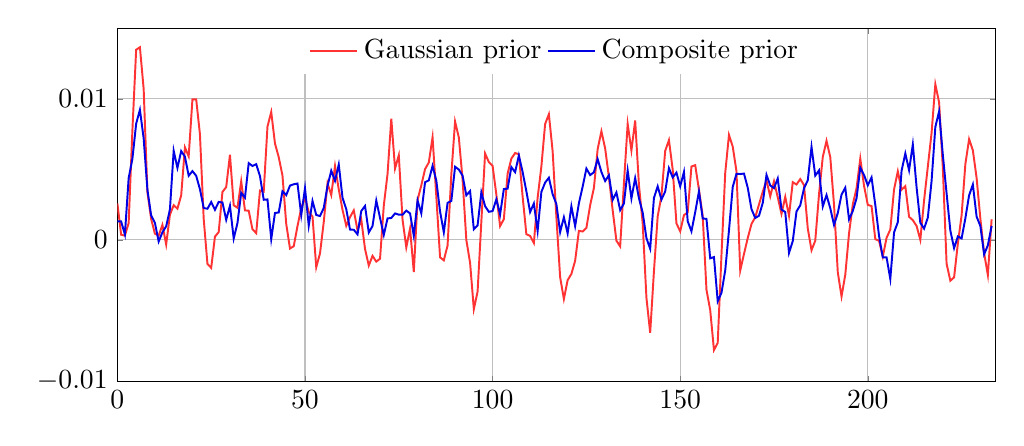
\begin{tikzpicture}
    \begin{axis}[
height=.5\linewidth, width=1.05\linewidth,
tickwidth=2pt,
          xmin=0, xmax=234,
          ymin=-0.01, ymax=0.015,
          xtick={0,50,100,150,200},
enlarge x limits=false,
          xmajorgrids,ymajorgrids,
          legend style={
              at={(0.5,1.0)},
              draw=none,
              anchor=north,
              legend columns=3,
              legend cell align={left},
          },
]
\addplot[color=red!80,line width=.7pt] table{
0 0.00258122824162351
1 0.000368601254411545
2 0.00030745958605436
3 0.00119417401771724
4 0.00777805080928041
5 0.0134726448785235
6 0.0136528719142471
7 0.0106992816247957
8 0.00337632144182029
9 0.00148286697584736
10 0.000439763792666876
11 0.000304600448526334
12 0.00106349047763005
13 -0.000324579331037332
14 0.00178440490805265
15 0.00245756974091439
16 0.00221565288985188
17 0.0031516285064734
18 0.00655940815298788
19 0.00592207341779099
20 0.00995362560449441
21 0.0099636363801736
22 0.00748760853573563
23 0.00149744237757917
24 -0.00169722943785065
25 -0.00197907237537272
26 0.000231109067595853
27 0.000556637568924161
28 0.00340069467950718
29 0.00374526431363804
30 0.00603566795628815
31 0.00245723892765046
32 0.00227893335331877
33 0.00415907909484973
34 0.00209336955243817
35 0.00206988372142582
36 0.000752043677412207
37 0.000482737466418646
38 0.00350050484336697
39 0.00342164618554783
40 0.00803246871098134
41 0.00906612482242754
42 0.00683010745152758
43 0.00586027266778076
44 0.00456174981450725
45 0.00113151294971819
46 -0.000608937789957465
47 -0.000445739910486282
48 0.000979662376905112
49 0.00226140370757009
50 0.00299185102064707
51 0.00197228416696256
52 0.00166313205220366
53 -0.00193514996395069
54 -0.000953115806749362
55 0.00127304620694461
56 0.0040092212007213
57 0.0031776805644975
58 0.00523927861874307
59 0.00358099672360581
60 0.00213503770995002
61 0.00100140500848893
62 0.00161534635626752
63 0.00209584331797023
64 0.000675418926775611
65 0.00144300700441301
66 -0.00064114700743773
67 -0.00181407664842344
68 -0.00112903551535389
69 -0.0015366105349963
70 -0.00133079273479052
71 0.00243253510562502
72 0.00467351094934684
73 0.00858765038317597
74 0.00506252220235662
75 0.00600033601264112
76 0.00143171179539717
77 -0.000534102249867846
78 0.00080894889264945
79 -0.00227074126792221
80 0.00282616084838496
81 0.00387024834790951
82 0.00501711917255847
83 0.00548864472013392
84 0.00727451117679352
85 0.00307821092484466
86 -0.0012321248634361
87 -0.00144716889197237
88 -0.000394311336778558
89 0.00464043448200586
90 0.00838474947542374
91 0.00726189979333043
92 0.0042742409740172
93 8.16900799051612e-07
94 -0.00162000855712347
95 -0.00490571684382318
96 -0.00366183442388747
97 0.00129260532616972
98 0.00612584000619665
99 0.00551774589531899
100 0.0052476154555462
101 0.00321312506467602
102 0.000981072882016261
103 0.00147290058668661
104 0.00469081235362065
105 0.00576497711599556
106 0.00615669463313797
107 0.00607058112445162
108 0.00308465710454367
109 0.000404861843821865
110 0.000284694420111902
111 -0.000217219854670986
112 0.00298334386078148
113 0.00520330915124047
114 0.00821363953266821
115 0.00890475381934428
116 0.00629404628383874
117 0.0016220700553319
118 -0.00263716341064058
119 -0.00419015350139193
120 -0.00284960831512125
121 -0.00240853946566148
122 -0.00147687917209973
123 0.000642232363694452
124 0.000597979498676542
125 0.000847304744741857
126 0.00245635624528021
127 0.00368035411464417
128 0.00643100142186806
129 0.00769864130049503
130 0.00648065902748977
131 0.00444995337832603
132 0.00210955247282462
133 -5.36202159603401e-05
134 -0.000461166053836081
135 0.00398211456327421
136 0.00821674352593272
137 0.00633764848473917
138 0.00846357484750415
139 0.00390750641423657
140 0.00118998913585248
141 -0.00409221560707513
142 -0.00658014964789467
143 -0.00223457357846512
144 0.00167333941799237
145 0.00311375682495411
146 0.00630432139491741
147 0.00707282782205155
148 0.00498933601201967
149 0.00117747536608222
150 0.000605515759768727
151 0.00175489377534118
152 0.00195477873361894
153 0.00520475511019488
154 0.00529605253372346
155 0.00355589705084893
156 0.00169224938376007
157 -0.00352727155280917
158 -0.00497183881166844
159 -0.00780537198315137
160 -0.0072963290672059
161 -0.00107939959417979
162 0.00473995986764768
163 0.00743989101547155
164 0.00661135748120487
165 0.00486440927444694
166 -0.00217311074504955
167 -0.000994732479872686
168 0.000127784031258465
169 0.00112809737143087
170 0.00160419143021123
171 0.00251181216994371
172 0.00341276805562122
173 0.00421372859423366
174 0.00307863456981628
175 0.00415024939531111
176 0.00302055029609451
177 0.0018462526482652
178 0.00304697933706747
179 0.0017072204807556
180 0.004092565829962
181 0.00392829350835764
182 0.00431221386359949
183 0.00388300501024032
184 0.000818398866901534
185 -0.000728574302554614
186 -5.19886603764521e-05
187 0.00323887384476273
188 0.00587528585920649
189 0.00702262450864692
190 0.00586617589456125
191 0.00249326606415404
192 -0.00228519862989882
193 -0.00400554354780943
194 -0.00246273080175774
195 0.000462809211187776
196 0.00251502225378151
197 0.00366348758566076
198 0.00576109568913474
199 0.00383025811341088
200 0.00248345487685684
201 0.00239953165324944
202 5.25261473676456e-05
203 -5.75324673997369e-05
204 -0.00118327055207105
205 0.00014949579707436
206 0.000736888109584802
207 0.00358416069128149
208 0.00486050372802046
209 0.00355506990605239
210 0.0038093557051499
211 0.00163736411726636
212 0.00140229613135042
213 0.000989623223350014
214 4.70751683413084e-06
215 0.00279347012241645
216 0.00518757685596242
217 0.00759278639008707
218 0.0110299248375648
219 0.00975227193755191
220 0.00510888517461388
221 -0.00168359557080876
222 -0.00288988396431369
223 -0.00265178516103962
224 -0.000260402753368046
225 0.00173744744946369
226 0.00536513083058566
227 0.00714240240837201
228 0.00635034115307416
229 0.00439460279390305
230 0.00151580757249164
231 -0.000927097016103267
232 -0.00248790337070212
233 0.00146322607498165
      };
\addplot[color=blue!90!black,line width=.7pt] table {
0 0.00131124952327494
1 0.0013083171585007
2 0.000387467273040757
3 0.00437640482473779
4 0.00574588024068226
5 0.00823450417235078
6 0.0092189955886847
7 0.00719583015317842
8 0.00356245601687925
9 0.00173097522720679
10 0.00121142923516294
11 -0.000111168945009787
12 0.0005373836086288
13 0.000963275070803791
14 0.00216148374964691
15 0.00632311330974771
16 0.00510052531560717
17 0.00629857287176371
18 0.00590041791414035
19 0.00454888894925217
20 0.00487511891400627
21 0.00454375893742048
22 0.00359259000412793
23 0.00226283554135322
24 0.00220948194615333
25 0.00268557140906978
26 0.00213894863993653
27 0.00269160414354214
28 0.00265313901532273
29 0.0014264696966603
30 0.00241988289172338
31 9.87085137533056e-05
32 0.0011922292258597
33 0.00333506335606695
34 0.00299826168983972
35 0.00544205041279357
36 0.00523791749064978
37 0.00536642791469501
38 0.00452127544734513
39 0.00284587981020005
40 0.00287070026552101
41 6.04712476220057e-05
42 0.00190805107684299
43 0.0019442116474583
44 0.0034529716858469
45 0.00317567102139161
46 0.00384812618806088
47 0.00394443601915017
48 0.00399681133641218
49 0.00175268860836574
50 0.00366380818911315
51 0.00101781372950288
52 0.00275994625524932
53 0.00176913076638136
54 0.00169236808159385
55 0.00226655823704301
56 0.00381861744721706
57 0.00490818884278191
58 0.00419085634382426
59 0.00534422743584424
60 0.00298525547514316
61 0.00217461714390609
62 0.000736089252435618
63 0.000718180118653476
64 0.000397033143204785
65 0.00204927537996731
66 0.00240627571088231
67 0.000526650580353283
68 0.000985945142104493
69 0.00279232830553601
70 0.00156226258225496
71 0.000353483062003521
72 0.00152540994868533
73 0.00155545262038315
74 0.00187715406125153
75 0.00178842134908095
76 0.00178520012848921
77 0.00207725532990922
78 0.00187864880411058
79 0.000291536008992694
80 0.00279481818592597
81 0.0018841870801331
82 0.00409026245010306
83 0.00422099110943562
84 0.00524724048598953
85 0.00420787078350331
86 0.00201301915786931
87 0.000540709181630539
88 0.00262662117572934
89 0.00276259167409092
90 0.00518491137386357
91 0.00498643788874098
92 0.00455436070952823
93 0.00316050896292299
94 0.00346464576928833
95 0.000755029995441592
96 0.00103472264962795
97 0.00337118441827349
98 0.00239013417319273
99 0.00199231979031212
100 0.00204558529860246
101 0.00287771448609839
102 0.00181439889045703
103 0.00360670949644179
104 0.00362955517157157
105 0.00516453036144701
106 0.00480201624286273
107 0.00597943112590585
108 0.00481964656180607
109 0.00344763610237106
110 0.0019767869068606
111 0.00258121038092675
112 0.000629296107488301
113 0.00340174320965524
114 0.00406284280237047
115 0.00440763422236425
116 0.00324035912122278
117 0.00254611202155947
118 0.000558579099857918
119 0.00160410862439271
120 0.000464768003687115
121 0.00238229032794348
122 0.000982246552164293
123 0.00259942670509454
124 0.00377163561325405
125 0.00505670061075531
126 0.00459441794155696
127 0.00479682765726346
128 0.00572743527241758
129 0.00481340188113763
130 0.00417311866567376
131 0.00458718171036151
132 0.00283643826903504
133 0.00336524066678294
134 0.00211108655288119
135 0.0025808862783572
136 0.00491861399576347
137 0.00293787742853964
138 0.00437639540285899
139 0.00295695552400108
140 0.00194087095094199
141 0.000132282760077025
142 -0.000626986725399561
143 0.00297469542316299
144 0.00379595462360203
145 0.00285589497976252
146 0.00343604911581855
147 0.00508117958375602
148 0.00443154329708131
149 0.00477070692267524
150 0.00379675778918638
151 0.00481367028629168
152 0.0013219947448534
153 0.000613244577811725
154 0.00196439159774042
155 0.00343608930854552
156 0.00151893402310433
157 0.00148985934940686
158 -0.00130648673898468
159 -0.00121698409394503
160 -0.00434966564703735
161 -0.00374710499269346
162 -0.00216618455396127
163 0.000675013663534883
164 0.00375185073187785
165 0.00468446413047053
166 0.00466894763424137
167 0.00470079206093448
168 0.00370429314078052
169 0.00218225182257164
170 0.00155560291241205
171 0.00171236456262947
172 0.00261799632543513
173 0.0046085915015407
174 0.00385785322028201
175 0.0036680944039929
176 0.00435403425813222
177 0.00215507131419573
178 0.00197471816337201
179 -0.000920784265770996
180 -8.46243260342858e-05
181 0.00201881879379415
182 0.00245426798287481
183 0.00366132854725286
184 0.00422050344255009
185 0.00658826384915529
186 0.00455554276976803
187 0.00492455197068406
188 0.00237517196367992
189 0.00318103150077402
190 0.00224057712363747
191 0.00106121934987819
192 0.00190239491029427
193 0.00321261411160265
194 0.00369868961343229
195 0.00145591427153803
196 0.00204809567833896
197 0.00295042297106041
198 0.00512080852271306
199 0.00459845309104483
200 0.00386979781345345
201 0.00442829140771209
202 0.00248212501405975
203 0.000278271427379488
204 -0.00124336464549463
205 -0.00123521916954482
206 -0.00276677109129166
207 0.0005363960203845
208 0.0012553854191359
209 0.00489885598290975
210 0.00612411252295922
211 0.00493917288954403
212 0.00676752437521581
213 0.00374052992193339
214 0.00121589096000715
215 0.000802647264024766
216 0.00158174743356588
217 0.00417398008331379
218 0.00800237993846591
219 0.00909736108648597
220 0.0060263290892223
221 0.00329626061540727
222 0.000664101071831226
223 -0.000579952073226018
224 0.000244875659525956
225 0.000108310918600181
226 0.00152724103088789
227 0.0031615711780128
228 0.00392270510929315
229 0.00165300672587535
230 0.000991144372434628
231 -0.00102428953920827
232 -0.00037941412944741
233 0.000988948721814708
      };
      \legend{Gaussian prior,Composite prior}
    \end{axis}
    \end{tikzpicture}
 

    \captionof{figure}{Differences in NDCG@100 for a random user as a function of the training iteration.}
    \label{fig:embed}\vspace{-1.0cm}
\end{figure}

\subsection{Ablation study and negative results}

In order to demonstrate that each of the new features we introduced for \emph{RecVAE} compared to \emph{Mult-VAE} indeed helps to improve performance, we have performed a detailed ablation study, comparing various subsets of the features:
\begin{inparaenum}[(1)]
\item new encoder architecture,
\item composite prior for the latent codes,
\item  rescaling,
\item alternating training, and 
\item removing denoising for the decoder.
\end{inparaenum}

Numerical results of the ablation study are presented in Table~\ref{tab:analysis}. We see that each new feature indeed improves the results, with all proposed new features leading to the best NDCG@100 scores on all three datasets. Some new features are complementary: e.g.,  rescaling and alternating training degrade the scores when applied individually, but together improve them; the new architecture does not bring much improvement by itself but facilitates other new features;  rescaling is dataset-sensitive, sometimes improving a lot and sometimes doing virtually nothing.

We have also performed extended analysis of the composite prior, namely checked how the  regularizer that brings variational parameters closer to old ones affects model stability. This regularizer stabilizes training, as evidenced by the rate of change in the variational parameters.
Figure~\ref{fig:embed} illustrates how the composite prior fixes the ``forgetting'' problem. It shows how NDCG@100 changes for a randomly chosen user as training progresses: each value is the difference in NDCG@100 for this user after each subsequent training update. Since each update changes the encoder network, it changes all user embeddings, and the changes can be detrimental for some users; note, however, that for the composite prior the changes remain positive almost everywhere while a simple Gaussian prior leads to much more volatile behaviour.

In addition, we would like to report the negative results of our other experiments. First, autoencoder-based models replace the matrix of user embeddings with a parameterized function, so it was natural to try to do the same for item embeddings. We trained \emph{RecVAE} with a symmetric autoencoder that predicts top users for a given item, training it alternately with regular \emph{RecVAE} and regularizing the results of each encoder with embeddings from the other model. The resulting model trained much slower, required more memory, and could not reach the results of \emph{RecVAE}.

Second, we have tried to use more complex prior distributions. Mixtures of Gaussians and the variational mixture VampPrior~\cite{tomczak2018vae} have (nearly) collapsed to a single node in our experiments, an effect previously noted in reinforcement learning~\cite{DBLP:journals/corr/abs-1809-10326}. The RealNVP prior~\cite{DBLP:conf/iclr/DinhSB17} has yielded better performance compared to the standard Gaussian prior, but we have not been able to successfully integrate it into the proposed composite prior: the composite prior with a Gaussian term remained the best throughout our experiments. We note this as a potential direction for further research.

Third, instead of -VAE-like weighing of KL divergence, we tried to re-weigh each of the terms in the decomposed KL divergence separately. It appears natural to assume that ``more precise'' regularization could be beneficial for both performance and understanding. However, neither a simple decomposition into entropy and cross-entropy nor the more complex one proposed in \cite{chen2018isolating} has led the model to better results.

\section{Conclusion}\label{sec:conclusion}

In this work, we have presented a new model called \emph{RecVAE} that combines several improvements for the basic \emph{Mult-VAE} model, including a new encoder architecture, new composite prior distribution for the latent codes, new approach to setting the hyperparameter , and a new approach to training \emph{RecVAE} with alternating updates of the encoder and decoder. As a result, performance of \emph{RecVAE} is comparable to EASE and significantly outperforms other models on classical collaborative filtering datasets such as \emph{MovieLens-20M}, \emph{Netflix Prize Dataset}, and \emph{Million Songs Dataset}.

We note that while we have provided certain theoretical motivations for our modifications, these motivations are sometimes incomplete, and some of our ideas have been primarily motivated by practical improvements. We believe that a comprehensive theoretical analysis of these ideas might prove fruitful for further advances, and we highlight this as an important direction for future research.

\FloatBarrier

\begin{acks}
This research was done at the Samsung-PDMI Joint AI Center at PDMI RAS and was supported by Samsung Research.
\end{acks}

\bibliographystyle{ACM-Reference-Format}
\bibliography{sample-base}

\appendix

\section{Network architecture}

\begin{figure}[h]
  \centering
  \includegraphics[width=.57\linewidth]{vae-mf_encoder}
  \caption{Architecture of the inference network .}
  \label{fig:encoder}
\end{figure}

\end{document}
